\documentclass[11pt,a4paper,titlepage]{article}
\usepackage[utf8]{inputenc}
\usepackage[left=1.5cm,text={18cm, 25cm},top=2.5cm]{geometry}
\usepackage{setspace}
\usepackage{graphicx}
\usepackage[czech]{babel}
\usepackage{caption}
\usepackage{subcaption}
\usepackage{subfig}
\usepackage{float}
\setlength{\parindent}{0cm}
\setlength{\parskip}{1em}
\sloppy

\begin{document}

    \section{Rozbor a analýza algoritmu bucket sort}
        Algoritmus bucket sort řadí pomocí stromu procesů. Vstupem algoritmu je řada čísel.
        Nechť $n$ je počet čísel v~této řadě, potom strom procesů obsahuje právě $m$ listových
        procesů, kde $m = \log_2 n$. Každý z~těchto procesů řadí část vstupu pomocí některého
        ze sekvenčních řadících algoritmů. Počet prvků, které tyto procesy řadí je tedy roven $\frac{n}{m}$.
        Dále nechť $p$ reprezentuje celkový počet procesů, potom $p = (2 \times \log_2 n) - 1$.
        Procesy, které nejsou listovými procesy, spojují dvě seřazené sekvence pomocí
        sekvenčního algoritmu.

        \subsection{Složitost a cena algoritmu}
        Listové procesy čtou $\frac{n}{\log_2 n}$ prvků. Jedná se tedy o~složitost $\mathcal{O}(\frac{n}{\log_2 n})$.
        Při použití sekvenčního řadícího algoritmu se složitostí $\mathcal{O}(r \times \log_2 r)$ bude výsledná složitost
        řazení $\mathcal{O}(\frac{n}{\log_2 n} \times \log_2 \frac{n}{\log_2 n}) = \mathcal{O}(n)$. Dále se zde nachází
        nelistové procesy, které je třeba do celkové složitosti algoritmu započítat. Proces při $j$--té iteraci se nachází
        v~úrovni stromu $i = (\log_2 m) - j$ a spojí 2 posloupnosti o~délce $\frac{n}{2^i}$. Při použití sekvenčního řadícího
        algoritmu určeného ke sloučení 2 seřazených posloupností se složitostí $\mathcal{O}(k)$ bude výsledná časová složitost
        práce nelistových procesů:
        $$\sum_{i=1}^{(\log_2 m) - 1} \frac{k \times n}{2^i} = \mathcal{O}(n)$$
        Poslední řazení kořenovým procesem s~uložením dat do paměti má složitost $\mathcal{O}(n)$.

        Celková časová složitost algoritmu je tedy $\mathcal{O}(n)$. Počet potřebných procesů k~dosažení této
        časové složitosti je $\mathcal{O}(log_2 n)$. Výsledná cena algoritmu bucket sort potom bude $\mathcal{O}(n \times log_2 n)$.
        Vzhledem k~časové složitosti sekvenční implementace algoritmu bucket sort se jedná o~optimální cenu.

	\section{Implementace}
        Aplikace \texttt{bks} řadí data ze souborů. Tyto soubory považuje za binární a každý byte dat je brán jako číslo vtupní sekvence.
        Aplikace tedy pracuje s~rozsahem čísel 0 -- 255. Načtená data ze souboru následně seřadí pomocí algoritmu bucket sort,
        kde je v~listových procesech použit sekvenční řadící algoritmus shell sort a~v~nelistových procesech je použit
        merge sort pro sjednocení 2 seřazených posloupností.

        Samotná aplikace \texttt{bks} přijímá 1 argument reprezentující vstupní soubor (výchozí hodnota je \texttt{numbers}) a lze ji spustit například pomocí následujícího příkazu:
\begin{verbatim}
mpirun --prefix /usr/local/share/OpenMPI -np PROCESS_COUNT bks INPUT_FILE
\end{verbatim}
        Při spuštění aplikace je nutné zadat správný počet procesů, jinak aplikace končí s~návratovou hodnotou 2.
        Počet procesů je určen nejbližší větší druhou mocninou čísla $\left \lceil{log_2 n}\right \rceil$.
        Důvodem této úpravy algoritmu je fakt, že $log_2 n$ je celé číslo, pokud je hodnota $n$ druhou
        mocninou čísla $2$. Ve chvíli, kdy $log_2 n$ nevychází jako celé číslo je i uměle navýšena velikost vstupního
        souboru o~čísla $255$ (maximální velikost jedné vstupní hodnoty) tak, aby všechny listové procesy pracovaly se stejnou
        velikostí dat. Kořenový proces, který provádí poslední řazení, poté takto přidaná čísla ignoruje.

	\section{Experimenty}
        Pro demonstraci algoritmu byl program spuštěn 100x nad krátkými náhodnými sekvencemi (řádově tisíce čísel) a 20x nad dlouhými náhodnými sekvencemi čísel (řádově desítky milionů).
        Výsledný čas zpracování byl měřen pomocí knihovní metody MPI\_Wtime. Měření probíhalo na jednom stroji s~procesorem Core i5-7300HQ (2.5GHz).

        U~krátkých posloupností algoritmus nedosáhl očekávané lineární časové složitosti. Důvodem takového časového průběhu může být skutečnost, že velikost dat, které řadí jednotlivé listové procesy pomocí shell sortu je příliš malá na stabilní časový průběh algoritmu. Svou roli zde může hrát i
        doba přístupu do paměti, zejména přítomnost dat v~paměti cache.

        U~delších sekvencí průběh zpracování odpovídá přibližně očekávané lineární složitosti a to i přesto, že pro řazení listovými procesy nebyl zvolen
        algoritmus se složitostí $\mathcal{O}(n \times \log_2 n)$. Složitost shell sortu je $\mathcal{O}(n^\frac{4}{3})$, což je (pokud se nejedná o~extrémní případy) velmi podobná složitost a proto v~těchto případech nemá tak veliký dopad.

        \begin{figure}[htbp]
            \begin{minipage}{.5\textwidth}
                \centering
                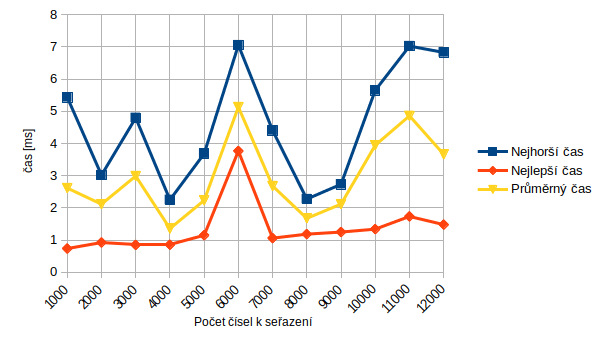
\includegraphics[width=1\linewidth]{small.png}
                \caption{Krátké sekvence náhodných čísel}
            \end{minipage}
            \begin{minipage}{.5\textwidth}
                \centering
                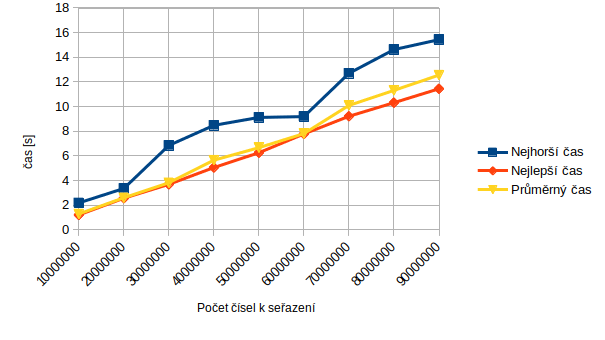
\includegraphics[width=1\linewidth]{big_numbers.png}
                \caption{Dlouhé sekvence náhodných čísel}
            \end{minipage}
        \end{figure}

	\section{Komunikace}
        Komunikaci začíná kořenový proces odesláním velikosti vstupního souboru všem procesům. Na základě této velikosti souboru a ID procesu, si každý
        proces určí od koho bude přijímat kolik dat, jakým algoritmem bude řadit (merge/shell sort) a komu bude posílat seřazená data. Kořenový proces
        následně načte celý soubor do paměti,  a pokud by měl poslední listový proces dostat
        méně dat než ostatní, doplní několik čísel s~hodnotou 255 na konec sekvence. Data následně odešle listovým procesům. Poté čeká, než mu procesy s~ID 1 a 2
        pošlou dvě seřazené posloupnosti. Pokud je na vstupu příliš málo čísel (méně než 3), provádí veškeré řazení kořenový proces.

        \begin{figure}[H]
            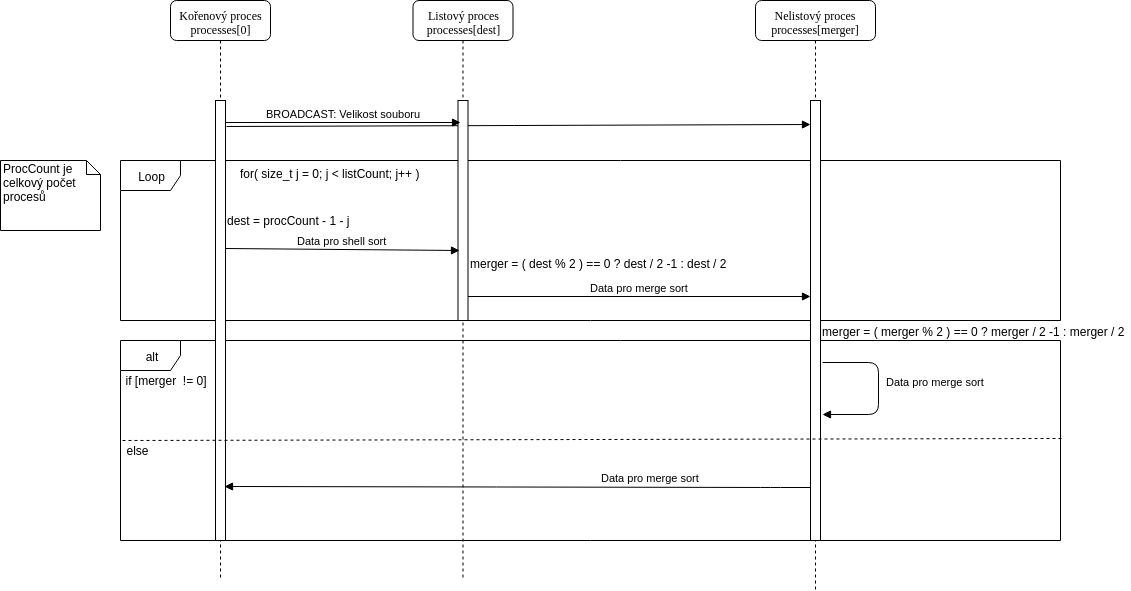
\includegraphics[width=1\linewidth]{sequenceDiagram.png}
            \caption{Komunikace mezi procesy}
        \end{figure}

	\section{Závěr}
        Výsledný algoritmus bucket sort má očekávanou lineární časovou složitost, ale trvá poměrně dlouho, než se časový průběh řazení stane stabilním. Tato
        implementace algoritmu bucket sort pracuje vždy s~vyváženým stromem procesů, a proto ne vždy listový a celkový počet procesů odpovídá vzorcům
        uvedených v~úvodu tohoto projektu.

\end{document}
